% Created 2017-04-17 Mon 02:13
\documentclass[10pt]{article}
\usepackage[utf8]{inputenc}
\usepackage[T1]{fontenc}
\usepackage{fixltx2e}
\usepackage{graphicx}
\usepackage{longtable}
\usepackage{float}
\usepackage{wrapfig}
\usepackage{rotating}
\usepackage[normalem]{ulem}
\usepackage{amsmath}
\usepackage{textcomp}
\usepackage{marvosym}
\usepackage{wasysym}
\usepackage{amssymb}
\usepackage{hyperref}
\tolerance=1000
\usepackage[a4paper,margin=3cm,footskip=.5cm]{geometry}
\usepackage{listings}
\usepackage{amsmath}
\author{Max Lam, Edward Look, Jesslynn Whittell}
\date{}
\title{SparsifyGradients - Reducing the Network Load by Dropping Gradient Values}
\hypersetup{
  pdfkeywords={},
  pdfsubject={},
  pdfcreator={Emacs 24.3.1 (Org mode 8.2.10)}}
\begin{document}

\maketitle

\section{Abstract}
\label{sec-1}

We present SparsifyGradients, a simple algorithm to drop 90\% of
gradient values during distributed machine learning training. We show
that the increase in network performance by dropping these values
outweigh the loss in precision, leading to an overall speedup in
training. We show up to 2x speedup over non-sparsified training on 14
c3.xlarge EC2 machines on training a cuda-convnet neural network for
the cifar10 image classification task.

\section{Introduction}
\label{sec-2}

Machine learning models, in particular deep neural networks, have
achieved state of the art results in tasks such as object detection,
speech recognition, image classification, game playing and more. Due
to increasing amounts of data and the computationally intensive nature
of training deep neural networks, research has been conducted to
distribute the training of these models across multiple
machines. Various algorithms to do this have been proposed such as
bulk synchronous parallel training (BSP), stale synchronous parallel
training (SSP) and asynchronous training. A main issue inherent to all
these methods is data communication: gradients need to be
communicated between machines every iteration of the algorithm. Even
with a few machines, distributed training can be bottlenecked by the
network bandwidth of the cluster.
\\
\\
\begin{figure}[htb]
\centering
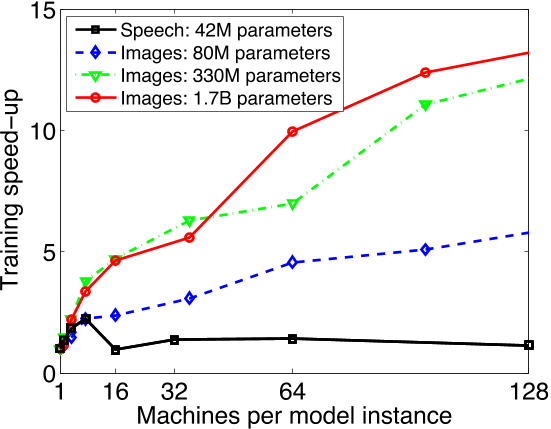
\includegraphics[width=0.5\textwidth]{./figures/figure1.png}
\caption{Speedup versus number of machines from "Large Scale Distributed Deep Networks" [Dean et al., NIPS 2012]. Scaling is limited by the network bandwidth with larger clusters.}
\end{figure}
\\
\\
In this project, we focus on tackling this communication issue. We
focus on the bulk synchronous parallel training algorithm in a cluster setting. The
following diagram describes the three phases of the bulk synchronous parallel algorithm.
\\
\begin{figure}[htb]
\centering
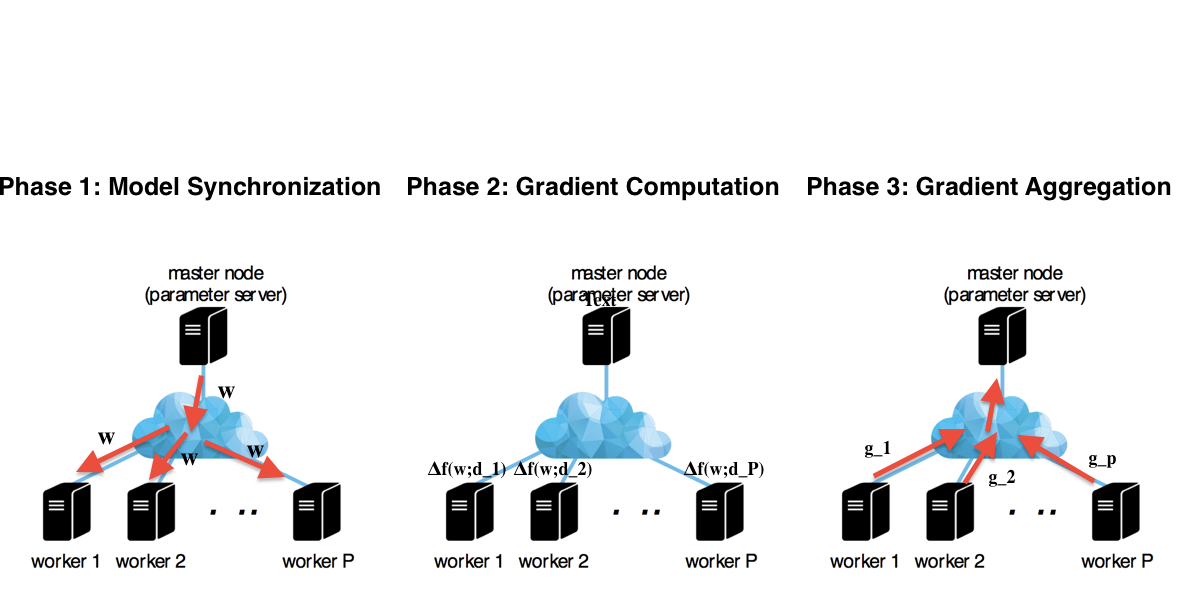
\includegraphics[width=0.8\textwidth]{./figures/figure2.png}
\caption{The bulk synchronous parallel training (BSP) algorithm. In phase 1 the model is distributed by the master to each worker in the cluster. In phase 2 each worker computes gradients given a shard of the overall data set with the model received from the master. In phase 3 gradients are sent by the workers back to the master to be aggregated and applied to the model. The process repeats.}
\end{figure}

\section{Sparsify Gradients}
\label{sec-3}

We call our proposed method SparsifyGradients, which does exactly that
-- zero out gradient values so that the overall gradient takes up less
memory and hence is faster to transmit across the network. Our belief
is that 90\% of the smaller gradient
values have little effect on convergence and can be discarded without
much penalty. During the gradient aggregation phase, SparsifyGradients
is performed on each gradient being communicated to the master,
zeroing out values of the gradient that fail to meet a certain threshold.
Specifically, gradient values are sorted by their absolute values and
dropped if they are below a specified percentile. For example, if
the percentile is specified to be 90, then 90\% of the gradient values with the smallest magnitudes
will be zeroed out. After applying SparsifyGradients
to each gradient being sent, the resulting gradients are then
converted to sparse format and communicated to the master.
\\
\\
\textbf{Sparsify Gradients Algorithm}
\begin{lstlisting}[language=Python,frame=lines]
def SparsifyGradient(gradient, percentile=90)
     threshold = calculate_percentile_value(abs(gradient), percentile)
     return sparse_format(gradient > threshold)
\end{lstlisting}

\section{Experimental Setup}
\label{sec-4}
We tested our algorithm on 14 c3.xlarge (13 workers, 1 master) Amazon
EC2 machines in a LAN setting, on a cuda-convnet style neural network
for the cifar10 task. The c3.xlarge machines are CPU instances with
7.5 GiB of memory and 4 virtual cpus, connected by a 500 Mbps network
channel. We use Tensorflow as a blackbox to evaluate and train the
neural network and MPI for communication between machines, which uses
the TCP protocol underneath. Our experiments compare sparsifying
gradients with a 90 percentile cutoff against the default
non-sparsified setting. We use a batch size of 8 per worker when
training the cuda convnet neural network.

\section{Results and Discussion}
\label{sec-5}

We achieve around a 2x speedup in time to .995 training accuracy on
training a cuda-convnet style neural network to perform the cifar10
image classification task. As expected, dropping 90\% of the gradient
values and converting to sparse format greatly reduces the time needed
to perform the gradient aggregation phase, which is mostly network
bandwidth bottlenecked. It is important to note that dropping 90\% of
values only decreases communication time by a factor of around 3-4 due
to the format of the sparse matrix, which stores indices along with
its values. Figure x compares the convergence properties of sparsified
vs non-sparsified distributed training. As expected, dropping gradient
values hurts convergence, though this loss in precision is compensated
by the speedup in network communication. It is interesting to note
that although 90\% of gradients' values are zeroed out, convergence to
99.5\% training accuracy is still achieved in a comparable number of
passes of data. We believe there are a couple of reasons for
this. Firstly, we believe that most gradient values do not change
model parameters too much and can be seen as noise. Figure x shows a
histogram of the absolute values of a gradient for the cuda convnet
model. As shown, most values are close to 0 and hence have a lesser
effect on the model. Secondly, we believe that if a gradient value
falls below the threshold in one iteration, but is essential to an accurate
model, then in a subsequent iteration the magnitude of that gradient
value will rise above the threshold to compensate. Further
investigation into these two points is future research.

\section{Conclusion}
\label{sec-6}

We present SparsifyGradients, a method which drops gradient values to
reduce network communication load. We tested our algorithm on a
cluster of 14 machines and trained a cuda-convnet model in a process
where 90\% of the lowest magnitude gradient weights are dropped. Doing
so achieves around 2x speedup over the default in time to 99.5\%
training accuracy. Finally, to explain the relative intactness of
convergence while dropping 90\% of gradient weights, we propose two
explanations. Firstly, that most gradient values are small and can be
seen as noise. Secondly, that important gradient values that fail the
threshold limit eventually succeed due to a delayed compensation mechanism.

\section{Future Work}
\label{sec-7}

It is very interesting that despite dropping 90\% of gradient values,
training still converges to a reasonable training accuracy (99.5\%). We
believe that this phenomena is the same as that which allows quantized
gradients to perform well despite the loss of data; it would be
interesting to investigate how much data loss can be tolerated while
also guaranteeing convergence. Furthermore, it would be interesting to
measure the impact of certain gradient values as they are propagated
among different weights. Investigating this might yield insight into which gradient values are worth keeping or discarding.
\\
\\
On the topic of quantization, further work can be done to reduce the
gradient network transfer overhead. Such extensions might include
quantizing the remaining values to 8-bits, or even enforcing some sort
of discretization.
\\
\\
We also neglected the network communication burden of the model
synchronization phase, which is in theory as expensive as the gradient
aggregation phase. Efficient communication of the model during this
phase is another topic for future work.
\\
\\
On the implementation side, it would be more efficient to use Tensorflow's native
distributed communication mechanism to test SparsifyGradient, as various scheduling optimizations (like prefetching)
are built into their system. Due to time and flexibility constraints we
opted to use MPI for communication and Tensorflow as an optimization black box.
\\
\\
Finally, as we have demonstrated that gradient values might be dropped
without much penalty, it would be interesting to implement the full
training procedure using UDP instead of TCP and simply ignoring the
lost packets. Due to time constraints and the complexity of managing a
lower level of the network model, we were not able to explore this.

\section{Code}
\label{sec-8}
\url{https://github.com/agnusmaximus/SparsifyGradients}
% Emacs 24.3.1 (Org mode 8.2.10)
\end{document}
